\documentclass[conference]{IEEEtran}
\usepackage{tikz}
\usetikzlibrary{positioning, arrows.meta, fit, shapes.multipart, calc}
\usepackage{amsmath}
\usepackage{amssymb}
\usepackage{listings}
\usepackage{xcolor}
\usepackage{booktabs}

\lstset{basicstyle=\ttfamily\scriptsize, breaklines=true, frame=single, framerule=0.2pt, backgroundcolor=\color{gray!5}}

\tikzset{
  block/.style={draw, rounded corners=2pt, minimum height=2.2em, minimum width=6em, align=center, font=\scriptsize},
  artifact/.style={block, fill=blue!8},
  process/.style={block, fill=orange!12},
  frozen/.style={block, fill=cyan!15, thick},
  human/.style={block, fill=red!10},
  head/.style={draw, rounded corners=1pt, minimum height=1.6em, minimum width=4.5em, align=center, font=\tiny, fill=green!10},
  arr/.style={-{Stealth[length=2mm]}, thick},
  darr/.style={arr, dashed},
  lbl/.style={font=\tiny, midway}
}

\title{A Frozen-Trunk Multi-Head Architecture for Citation-Fidelity Remediation via Positive-Unlabeled Learning}

\author{
\IEEEauthorblockN{Johnny~Morgan}
\IEEEauthorblockA{Information Systems, UMBC\\
yj07538@umbc.edu}
}

\begin{document}
\maketitle

\begin{abstract}
Customer products cite the requirements they satisfy, but citation is imperfect: not every record that meets a requirement is properly cited, so customers do not always receive products they are entitled to. We present a system that learns the discipline of attribution from deterministic citation labels and applies it predictively to text, surfacing uncited-but-relevant records for human adjudication. The architecture is a single domain-adapted transformer encoder (the \emph{trunk}), frozen after continued pretraining, serving fifty independently trained, independently versioned binary classification heads---one per customer. Labels derive deterministically from a requirements repository; because citations are incomplete, training is positive-unlabeled: positives are clean, negatives are contaminated with the very missed citations the system exists to find. High-confidence disagreements between model and labels enter a human-in-the-loop adjudication queue whose outcomes are simultaneously delivered corrections and label improvements, driving an iterative retraining cycle. The frozen-trunk contract makes that cycle cheap: heads retrain in seconds against cached embeddings. We define an operational cadence---monthly head retraining to reach and hold minimum viable product, annual trunk fine-tuning---with every dataset, label set, and model versioned and reproducible under a companion model-management architecture~[1].
\end{abstract}

\section{Introduction}
The operational problem is citation fidelity. Products are produced against customer requirements; the requirements satisfied are cited in the product record. Citation is deterministic where it occurs, but it is incomplete---some records that meet a requirement carry no citation, and the affected customer never receives that product. The deterministic citation record is therefore both the training signal and the defect to be remediated: we train a model on the attribution discipline the citations encode, then use it to predict attribution from text alone, flagging records the citations missed.

The system does not pursue perfection. Citation practice, requirements, and data all drift; the design goal is \emph{best sustained performance} under an iterative correction loop, not a fixed accuracy target. The architecture is built so that the frequent operations---head retraining after label corrections, requirement changes, or a new month of data---cost seconds, while the rare operation (trunk adaptation) is scheduled annually.

The system originates from a validated single-label baseline: \texttt{distilbart-mnli-12-3} fine-tuned on 25k labeled samples (98.3\% accuracy against citation labels), extended by domain-adaptive pretraining (DAPT) on $\sim$250k unlabeled records, then widened to fifty customer heads.

\section{Architectural Contract}
\begin{quote}
\emph{The trunk is frozen after DAPT. Its pooled embedding space is a fixed interface. Heads are pure consumers of that interface.}
\end{quote}
Consequences: (1)~heads share no trainable state, so retraining one cannot perturb another; (2)~the corpus is embedded once per trunk version and cached, so all head training is CPU-only and takes seconds; (3)~a head is valid only against the trunk version (and feature-set version, \S\ref{sec:aug}) it was trained on, recorded in metadata and enforced at load time.

\section{Architecture}
Fig.~\ref{fig:arch} shows inference. Text passes through the frozen encoder; the last hidden state is mean-pooled over non-pad tokens into $z \in \mathbb{R}^{1024}$. Each customer head $c$ computes $\hat{y}_c = \mathbb{1}[\sigma(w_c^\top z + b_c) > \tau_c]$ with a per-head calibrated threshold. Fifty predictions are written to fifty dataframe columns; one trunk pass yields fifty answers.

\begin{figure}[t]
\centering
\resizebox{\columnwidth}{!}{%
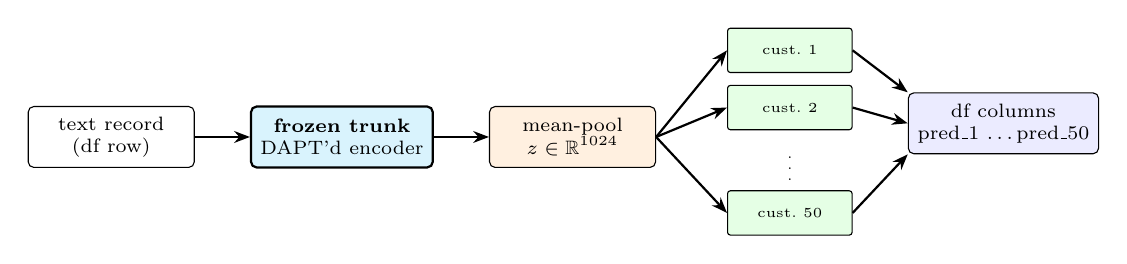
\begin{tikzpicture}[node distance=5mm and 7mm]
\node[block] (text) {text record\\(df row)};
\node[frozen, right=of text] (trunk) {\textbf{frozen trunk}\\DAPT'd encoder};
\node[process, right=of trunk] (pool) {mean-pool\\$z \in \mathbb{R}^{1024}$};
\node[head, right=9mm of pool, yshift=11mm] (h1) {cust.\ 1};
\node[head, below=1.5mm of h1] (h2) {cust.\ 2};
\node[below=0mm of h2, font=\tiny] (dots) {$\vdots$};
\node[head, below=0mm of dots] (h50) {cust.\ 50};
\node[artifact, right=7mm of h2, yshift=-2mm] (df) {df columns\\pred\_1 \dots pred\_50};
\draw[arr] (text) -- (trunk);
\draw[arr] (trunk) -- (pool);
\draw[arr] (pool.east) -- (h1.west);
\draw[arr] (pool.east) -- (h2.west);
\draw[arr] (pool.east) -- (h50.west);
\draw[arr] (h1.east) -- (df.north west);
\draw[arr] (h2.east) -- (df.west);
\draw[arr] (h50.east) -- (df.south west);
\end{tikzpicture}%
}
\caption{Inference dataflow: one GPU trunk pass, fifty customer heads as independent linear projections.}
\label{fig:arch}
\end{figure}

\section{Training Data Acquisition}
\label{sec:abc}
Three repositories supply training data (Fig.~\ref{fig:abc}):
\begin{itemize}
\item \textbf{A --- metadata repository.} A one-year pull defines the training population and supplies join IDs.
\item \textbf{B --- content repository.} Text content, joined to A by ID; this is what the trunk embeds.
\item \textbf{C --- requirements repository.} The label authority. Customer $c$'s requirements define a deterministic labeling function $L_c$: applied to each A+B record via the citations in the product record, it yields the label column for head $c$.
\end{itemize}
Every acquisition is a recorded \emph{recipe}---A query, time window, snapshot date, B join specification, and the C requirements version behind each $L_c$---registered in the model-management database~[1]. A dataset is reconstructable by re-executing its recipe; reproducibility means recipes re-execute, not that dataframes were kept. A change to customer $c$'s requirements in C is a new version of $L_c$, a new label-set version, and a seconds-scale retrain of head $c$: C is upstream of the deployment manifest.

Rollout is phased. Phase~1 proves the pipeline end-to-end on customer~1: pull, join, label, train, infer into the customer-1 column, validate. Phase~2 replicates the labeling across all fifty customers and trains fifty heads against cached embeddings; the phase-1 model remains registered as the comparison baseline.

\begin{figure}[t]
\centering
\resizebox{\columnwidth}{!}{%
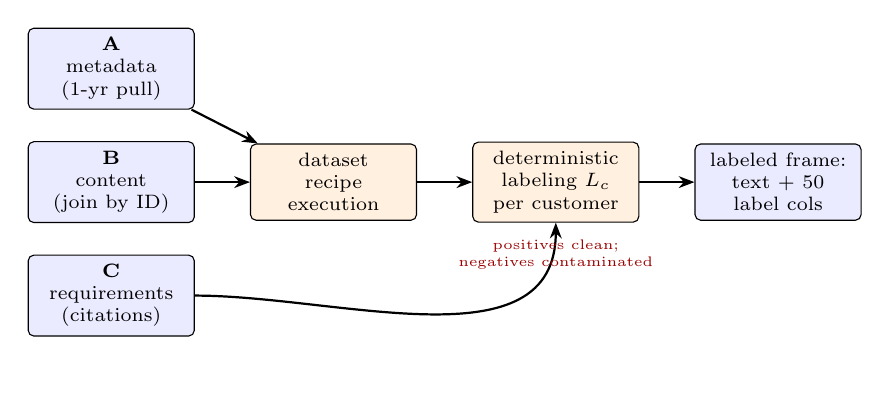
\begin{tikzpicture}[node distance=4mm and 7mm]
\node[artifact] (a) {\textbf{A}\\metadata\\(1-yr pull)};
\node[artifact, below=of a] (b) {\textbf{B}\\content\\(join by ID)};
\node[artifact, below=of b] (c) {\textbf{C}\\requirements\\(citations)};
\node[process, right=of b] (join) {dataset\\recipe\\execution};
\node[process, right=of join] (lab) {deterministic\\labeling $L_c$\\per customer};
\node[artifact, right=of lab] (df) {labeled frame:\\text + 50\\label cols};
\draw[arr] (a) -- (join);
\draw[arr] (b) -- (join);
\draw[arr] (c.east) to[out=0,in=-90] (lab.south);
\draw[arr] (join) -- (lab);
\draw[arr] (lab) -- (df);
\node[font=\tiny, below=1mm of lab, align=center, color=red!60!black] {positives clean;\\negatives contaminated};
\end{tikzpicture}%
}
\caption{A/B/C acquisition and deterministic labeling. Citations make positives reliable; missed citations contaminate the negatives.}
\label{fig:abc}
\end{figure}

\section{Positive-Unlabeled Learning and the Adjudication Loop}
\label{sec:pu}
Because citation is incomplete, the label set is positive-unlabeled: cited records are true positives; uncited records are a mixture of true negatives and missed citations---the latter being precisely the system's target discovery. Three consequences:

\textbf{Training.} Standard supervised training on the noisy labels is the pragmatic baseline; the text signal generalizes past citation gaps, so the model scores uncited-but-similar records high despite their negative labels. If contamination proves heavy, principled escalations exist (non-negative PU risk estimation with an estimated class prior; spy-based negative cleaning). Class imbalance is handled per head with weighted loss.

\textbf{Evaluation.} Accuracy against C's labels systematically understates the model where it matters most: a ``false positive'' is either a model error or a discovered missed citation, and only human judgment distinguishes them. Evaluation therefore scores against \emph{adjudicated} labels on sampled disagreements, and reported metrics carry their label-set version.

\textbf{Operation (Fig.~\ref{fig:loop}).} High-confidence disagreements enter a review queue. The adjudicator's decision is simultaneously product remediation and training signal: \emph{missed citation} $\rightarrow$ the customer receives the product and a label correction is recorded; \emph{model error} $\rightarrow$ a confirmed hard negative. Corrections form a versioned overlay on the deterministic label sets (C remains the untouched system of record); each overlay version triggers a seconds-scale head retrain. Customer feedback on delivered products enters the same queue, and recurring pathologies are traced back to training data through the recipe and lineage records~[1]. The loop does not converge to perfection and is not intended to; it holds the system at best achievable performance under drift.

\begin{figure}[t]
\centering
\resizebox{\columnwidth}{!}{%
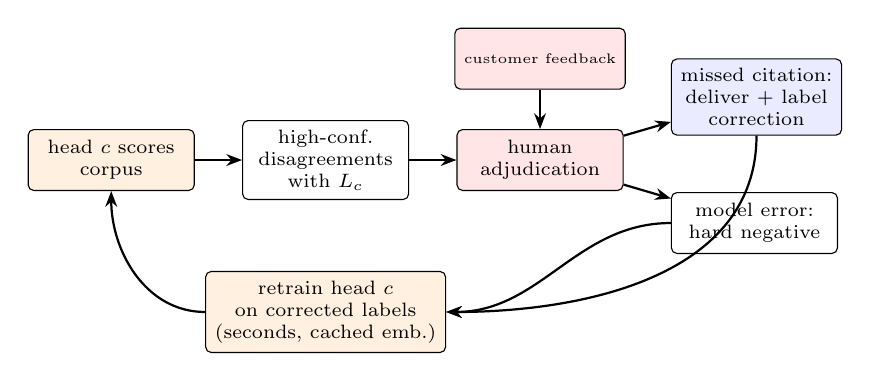
\begin{tikzpicture}[node distance=4mm and 6mm]
\node[process] (score) {head $c$ scores\\corpus};
\node[block, right=of score] (dis) {high-conf.\\disagreements\\with $L_c$};
\node[human, right=of dis] (adj) {human\\adjudication};
\node[artifact, right=of adj, yshift=8mm] (fix) {missed citation:\\deliver + label\\correction};
\node[block, right=of adj, yshift=-8mm] (err) {model error:\\hard negative};
\node[process, below=9mm of dis] (retrain) {retrain head $c$\\on corrected labels\\(seconds, cached emb.)};
\draw[arr] (score) -- (dis);
\draw[arr] (dis) -- (adj);
\draw[arr] (adj) -- (fix);
\draw[arr] (adj) -- (err);
\draw[arr] (fix.south) to[out=-90,in=0] (retrain.east);
\draw[arr] (err.west) to[out=180,in=0] (retrain.east);
\draw[arr] (retrain.west) to[out=180,in=-90] (score.south);
\node[human, above=5mm of adj, font=\tiny] (cust) {customer feedback};
\draw[arr] (cust) -- (adj);
\end{tikzpicture}%
}
\caption{HITL adjudication loop: each decision is both a delivered correction and a label improvement feeding the next retrain.}
\label{fig:loop}
\end{figure}

\section{Training Pipeline}
\textbf{Trunk (annual; GPU).} Continued pretraining uses BART's native text-infilling denoising objective (Poisson($\lambda{=}3$) spans, $\sim$30\% corruption) on the unlabeled corpus: fp16, learning rate $10^{-5}$--$5{\times}10^{-5}$, 1--3 epochs, sequence length capped to true field length, corpus deduplicated against all frozen test splits before training. The encoder is saved as \texttt{trunk/v$N$} and the corpus embedded once into a row-aligned cache.

\textbf{Heads (monthly and on-demand; CPU, seconds).} Fit against cached embeddings with weighted \texttt{BCEWithLogitsLoss}; sweep the decision threshold on validation; evaluate per-class precision/recall/F1 on the head's frozen test split against the current adjudicated label version; save \texttt{head.pt} + \texttt{meta.json} under the next version; bump the manifest. Rollback is a one-line manifest revert.

\section{Registry and Deployment}
Trunk, heads, thresholds, and the deployment manifest are filesystem artifacts under git, loaded at inference-session initialization with a hard trunk-version compatibility assertion per head. The full registry design---model cards, dataset recipes, label rules and correction overlays, lineage, and orchestration---is specified in the companion model-management architecture~[1]; this paper's deployment surface is the manifest it governs.

\section{Operational Cadence}
\label{sec:cadence}
\textbf{Monthly (MVP heartbeat).} Ingest the new month of A/B data; embed only new records (cache append); apply current label rules plus correction overlays; retrain all fifty heads; recalibrate thresholds; compare each head's metrics against its prior version (regression check); bump the manifest. Aggregate cost is minutes of CPU plus one small embedding job. Monthly iteration is the path to minimum viable product and the mechanism that holds it.

\textbf{Annual (trunk refresh).} Fine-tune or re-run DAPT on the grown corpus $\rightarrow$ \texttt{trunk/v$N{+}1$}; re-embed the full corpus; rebuild all fifty heads against the new cache; cut the manifest over atomically---trunk and all head versions in one commit. Annual review also revisits feature augmentation (\S\ref{sec:aug}) and PU escalation decisions.

All cadence runs execute as recorded, versioned training jobs; any model, monthly or annual, is reproducible by recipe re-execution~[1]. Fine-tuning from a prior model is first-class: parent lineage is recorded, so the model history forms a DAG.

\section{Feature Augmentation}
\label{sec:aug}
If text alone is insufficiently predictive for some customers, structured features from A (and derived signals) augment the representation without touching the trunk: $z' = [\,z \,;\, \phi(\text{metadata})\,]$, where $\phi$ is a versioned feature-extraction spec, and heads widen to $\mathbb{R}^{1024+d}$. The frozen-trunk contract extends naturally: a head is valid against a (trunk version, feature-set version) pair, both asserted at load. Feature sets are versioned artifacts with their own recipes, so augmentation preserves reproducibility.

\section{Failure Modes and Guards}
\begin{table}[h]
\scriptsize
\centering
\begin{tabular}{p{3.6cm} p{3.9cm}}
\toprule
\textbf{Failure} & \textbf{Guard} \\
\midrule
Missed citations trained as negatives & PU framing; disagreement mining + adjudication; correction overlay \\
Metrics flatter/blame the wrong thing & Evaluation against adjudicated labels, versioned with the label set \\
Stale-trunk (or stale-feature-set) head served & Load-time version assertions \\
Silent regression on monthly retrain & Per-head metric comparison $v_N$ vs $v_{N-1}$ before manifest bump \\
Test contamination via DAPT corpus & Pre-DAPT dedup against all frozen test splits \\
Imbalance masked by accuracy & Per-head F1/precision/recall mandatory \\
Requirements drift & C-versioned label rules; change $\Rightarrow$ label-set version $\Rightarrow$ head retrain \\
\bottomrule
\end{tabular}
\end{table}

\section{Discussion}
The design aligns three cycles at three costs: adjudication-driven corrections (continuous, seconds per retrain), monthly cadence (minutes, the MVP heartbeat), and annual trunk refresh (hours, scheduled). Each cycle's outputs are versioned artifacts with recorded lineage, so ``best performance'' is not a snapshot but a maintained state: the system is always as good as its latest adjudications, and always able to prove how it got there.

\begin{thebibliography}{1}
\bibitem{mm} J.~Morgan, ``A Recipe-Based Model-Management Architecture for Versioned, Reproducible Training,'' companion paper, 2026.
\end{thebibliography}

\end{document}
